\newpage
\subsection{QuizziPedia::Front-End::Services}
\begin{figure}[ht]
	\centering
	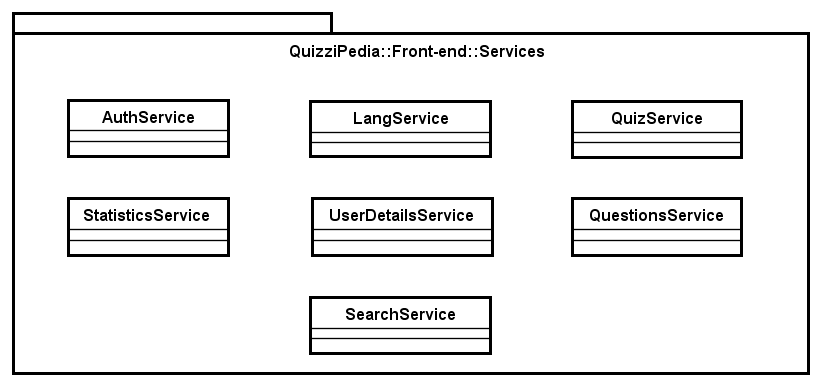
\includegraphics[scale=0.60]{UML/Package/QuizziPedia_Front-End_Services.png}
	\caption{QuizziPedia::Front-End::Services}
\end{figure} \FloatBarrier
\subsubsection{Informazioni generali}
\begin{itemize}
	\item \textbf{Descrizione}: package che contiene le classi individuate che permettono la comunicazione del lato front-end con il lato back-end;
	\item \textbf{Padre:} \texttt{Front-End};
	\item \textbf{Interazione con altri componenti:}
	\begin{itemize}
		\item \texttt{Models}: package che contiene le classi \textit{model\ped{G}} individuate;
		\item \texttt{Controllers}: package che contiene le classi \textit{controller\ped{G}} individuate.
	\end{itemize} 
\end{itemize}
\subsubsection{Classi}

\paragraph{QuizziPedia::Front-End::Services::AuthService}
\begin{figure}[ht]
	\centering
	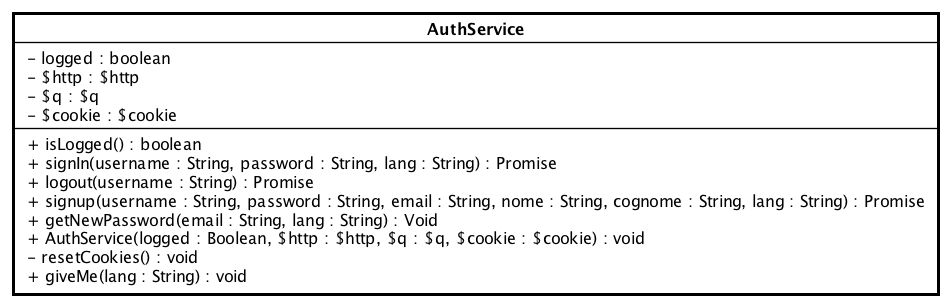
\includegraphics[scale=0.80]{UML/Classi/Front-End/QuizziPedia_Front-end_Services_AuthService.png}
	\caption{QuizziPedia::Front-End::Services::AuthService}
\end{figure} \FloatBarrier
\begin{itemize}
	\item \textbf{Descrizione}: questa classe permette di gestire la registrazione e l'autenticazione di un utente;
	\item \textbf{Utilizzo}: fornisce le funzionalità di registrazione e autenticazione ai controllers. Controlla che i dati inseriti dall'utente siano presenti nel \textit{Database\ped{G}} in caso di autenticazione. Presenta anche le funzionalità per la gestione del reset della password;
	\item \textbf{Relazione con altre classi:}
	\begin{itemize}
		\item \textit{OUT} \texttt{LoginController}: questa classe gestisce la logica alla base della pagina di autenticazione;
		\item \textit{OUT} \texttt{PasswordForgotController}: questa classe gestisce la logica alla base del reset della password;
		\item \textit{OUT} \texttt{SignUpController}: questa classe gestisce la logica alla base della registrazione di un nuovo utente.
	\end{itemize}
	\item \textbf{Attributi:}
	\begin{itemize}
		\item \texttt{-} \texttt{logged: Boolean} \\ Campo dati che indica se l'utente è autenticato;
		\item \texttt{-} \texttt{\$http: \$http} \\ Campo dati che contiene un riferimento al servizio \$http che permette la comunicazione con il protocollo \textit{HTTP\ped{G}};
		\item \texttt{-} \texttt{\$q: \$q} \\ Campo dati che contiene un riferimento a \$q, un servizio offerto da \textit{AngularJS\ped{G}} per la gestione, tramite \textit{Promise\ped{G}}, di chiamate asincrone;
		\item \texttt{-} \texttt{\$cookie: \$cookie} \\ Campo dati che consente di salvare il valore di logged ed evitare che venga richiesta l'autenticazione ad ogni ricaricamento della pagina.
	\end{itemize}
	\item \textbf{Metodi:}
	\begin{itemize}
		\item \texttt{+} \texttt{AuthService(logged: Boolean, \$http: \$http, \$q: \$q, \$cookie: \$cookie)} \\ Metodo costruttore della classe. \\
		\textbf{Parametri}:
		\begin{itemize}
			\item \texttt{logged: Boolean} \\ Parametro che indica se l'utente è loggato o no;
			\item \texttt{\$http: \$http} \\ Parametro contenente un riferimento al servizio \$http creato da \textit{AngularJS\ped{G}} per facilitare la comunicazione mediante protocollo \textit{HTTP\ped{G}};
			\item \texttt{\$q: \$q} \\ Parametro contenente un riferimento al servizio \$q creato da \textit{AngularJS\ped{G}} per facilitare la gestione di funzione asincrone mediante l’utilizzo delle \textit{Promise\ped{G}};
			\item \texttt{\$cookie: \$cookie} \\ Parametro che consente di salvare il valore di logged ed evitare che venga richiesta l'autenticazione ad ogni ricaricamento della pagina.
		\end{itemize}
		\item \texttt{+} \texttt{isLogged(): Boolean} \\ Metodo che restituisce il valore dell'attributo \textit{logged} salvato all'interno del cookie che permette di evitare di eseguire l'autenticazione ad ogni caricamento della pagina;
		 
		\item \texttt{+} \texttt{signIn(email: String, password: String): Promise}\\ Metodo che permette di effettuare il login all'applicazione facendo una richiesta di autenticazione al back-end passando i parametri ricevuti. Il metodo ritorna una \textit{Promise\ped{G}}. In caso la \textit{Promise\ped{G}} venga rifiutata, verrà restituito al \texttt{LoginController} un oggetto \texttt{ErrorModelInfo} contenente tutti i dettagli dell'errore. In caso la \textit{Promise\ped{G}} venga accettata, verrà restituito al chiamante del metodo il risultato della chiamata. \\
			\textbf{Parametri}: 
			\begin{itemize}
				\item \texttt{username: String} \\ Parametro che rappresenta lo username o la email dell'utente;
				\item \texttt{password: String} \\ Parametro che rappresenta la password dell'utente.
			\end{itemize}
			
		\item \texttt{+} \texttt{logout(username: String): Promise} \\ Metodo che permette di effettuare il logout dall'applicazione. Il metodo ritorna una \textit{Promise\ped{G}}. In caso la \textit{Promise\ped{G}} venga rifiutata, verrà restituito al \texttt{LogoutController} un oggetto \texttt{ErrorModelInfo} contenente tutti i dettagli dell'errore. In caso la \textit{Promise\ped{G}} venga accettata, verrà restituito al chiamante del metodo il risultato della chiamata.\\
		\textbf{Parametri}:
		\begin{itemize}
			\item \texttt{username: String} \\ Parametro che rappresenta l'utente che vuole eseguire il logout.
		\end{itemize}
		
		\item \texttt{+} \texttt{signup(username: String, password: String, email: String, nome: String, cognome: String): Promise} \\Metodo che permette di effettuare la registrazione all'applicazione tramite richiesta di creazione nuovo account al back-end. Il metodo ritorna una \textit{Promise\ped{G}}. In caso la \textit{Promise\ped{G}} venga rifiutata, verrà restituito al \texttt{SignUpController} un oggetto \texttt{ErrorModelInfo} contenente tutti i dettagli dell'errore. In caso la \textit{Promise\ped{G}} venga accettata, verrà restituito al chiamante del metodo il risultato della chiamata. \\
			\textbf{Parametri}:
			\begin{itemize}
				\item \texttt{username: String} \\ Parametro che rappresenta lo username o la email dell'utente;
				\item \texttt{password: String} \\ Parametro che rappresenta la password dell'utente;
				\item \texttt{email: String} \\ Parametro che rappresenta la email dell'utente;
				\item \texttt{nome: String} \\ Parametro che rappresenta il nome dell'utente;
				\item \texttt{cognome: String} \\ Parametro che rappresenta il cognome dell'utente.
			\end{itemize}
			
		\item \texttt{+} \texttt{getNewPassword(email: String): Void}  \\Metodo che permette il recupero della password. Il metodo ritorna una \textit{Promise\ped{G}}. In caso la \textit{Promise\ped{G}} venga rifiutata, verrà restituito al \texttt{PasswordForgotController} un oggetto \texttt{ErrorModelInfo} contenente tutti i dettagli dell'errore. In caso la \textit{Promise\ped{G}} venga accettata, verrà restituito al chiamante del metodo il risultato della chiamata. \\
			\textbf{Parametri}:
			\begin{itemize}
				\item \texttt{email: String} \\ Parametro che rappresenta la email a cui mandare un messaggio per resettare la password.
			\end{itemize}
	\end{itemize}
\end{itemize}
\paragraph{QuizziPedia::Front-End::Services::LangService}

\label{QuizziPedia::Front-End::Services::LangService}
\begin{figure}[ht]
	\centering
	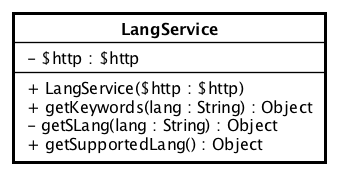
\includegraphics[scale=0.60]{UML/Classi/Front-End/QuizziPedia_Front-end_Services_LangService.png}
	\caption{QuizziPedia::Front-End::Services::LangService}
\end{figure}\FloatBarrier
\begin{itemize}
	\item \textbf{Descrizione}: questa classe permette di gestire la lingua nella quale si è scelto di utilizzare l'applicazione;
	\item \textbf{Utilizzo}: fornisce delle funzionalità per recuperare la giusta traduzione delle pagine;
	\item \textbf{Relazione con altre classi:}
	\begin{itemize}
		\item \textbf{IN \texttt{AppRun}}: classe che permette l'avvio dell'applicazione.
	\end{itemize}
	\item \textbf{Attributi}:
	\begin{itemize}
		\item \texttt{-} \texttt{\$http: \$http} \\ Campo dati che contiene un riferimento al servizio \$http che permette la comunicazione con il protocollo \textit{HTTP\ped{G}}.
	\end{itemize}
	\item \textbf{Metodi}:
	\begin{itemize}
		\item \texttt{+} \texttt{LangService(\$http: \$http)} \\ Metodo costruttore della classe; \\
		\textbf{Parametri}:
		\begin{itemize}
			\item \texttt{\$http: \$http} \\ Campo dati contenente un riferimento al servizio \$http creato da \textit{Angular\ped{G}} per facilitare la comunicazione mediante protocollo \textit{HTTP\ped{G}}.
		\end{itemize}
		\item \texttt{+} \texttt{getKeywords(lang: String): Object} \\Metodo che ritorna la lista di tutte le keywords nella lingua richiesta.\\
		\textbf{Parametri}:
		\begin{itemize}
			\item \texttt{lang: String} \\ Parametro che indica la lingua delle \textit{keywords\ped{G}} da restituire.
		\end{itemize}
	\end{itemize}
\end{itemize}
\paragraph{QuizziPedia::Front-End::Services::QuestionsService}

\label{QuizziPedia::Front-End::Services::QuestionService}
\begin{figure}[ht]
	\centering
	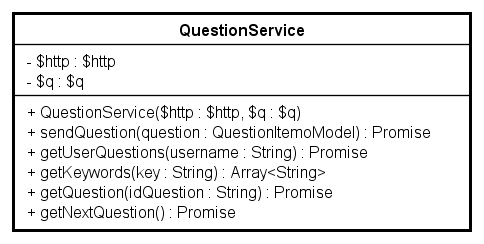
\includegraphics[scale=0.60]{UML/Classi/Front-End/QuizziPedia_Front-end_Services_QuestionService.png}
	\caption{QuizziPedia::Front-End::Services::QuestionService}
\end{figure}\FloatBarrier
\begin{itemize}
	\item \textbf{Descrizione}: questa classe permette di ottenere domande esistenti e salvare nuove domande;
	\item \textbf{Utilizzo}: utilizzata per richiedere domande presenti nel database. Offre inoltre delle funzionalità per inserire nuove domande;
	\item \textbf{Relazione con altre classi:}
	\begin{itemize}
		\item \textbf{IN \texttt{QuestionItemModel}}: rappresenta una domanda. Contiene tutte le informazioni necessarie alla
		presentazione del contenuto della domanda; 
		\item \textbf{IN \texttt{TrueFalseQuestionsController}}: questa classe permette di gestire la creazione e la modifica di una domanda vero/falso;
		\item \textbf{IN \texttt{MultiplyQuestionsController}}: questa classe permette di gestire la creazione e la modifica di una domanda a risposta multipla; 
		\item \textbf{IN \texttt{ConnectionQuestionsController}}: questa classe permette di gestire la creazione e la modifica di una domanda a collegamento;
		\item \textbf{IN \texttt{ImagesSortingQuestionsController}}: questa classe permette di gestire la creazione e la modifica di una domanda a ordinamento immagini;
		\item \textbf{IN \texttt{StringsSortingQuestionsController}}: questa classe permette di gestire la creazione e la modifica di una domanda a ordinamento di stringhe;
		\item \textbf{IN \texttt{FillingQuestionsController}}: questa classe permette di gestire la creazione e la modifica di una domanda a riempimento di spazi; 
		\item \textbf{IN \texttt{ClickableAreaQuestionsController}}: questa classe permette di gestire la creazione e la modifica di una domanda ad area cliccabile;
		\item \textbf{IN \texttt{EditorQMLController}}: questa classe permette di gestire la creazione e la modifica di domande create tramite editor QML;
		\item \textbf{IN \texttt{QuestionsManagementController}}: questa classe permette di gestire e di ottenere le domande create dall'utente;
		\item \textbf{IN \texttt{TopicKeywordsController}}: questa classe permette di gestire il recupero delle parole chiave di un questionario;
		\item \textbf{IN \texttt{QuestionnaireQuestionsManagementController}}: questa classe permette di gestire il recupero delle domande per il questionario;
		\item \textbf{IN \texttt{QuestionsController}}: questa classe permette di gestire il recupero delle domande per poterle stampare nella modalità allenamento;
		\item \textbf{IN \texttt{QuestionsItemModel}}: rappresenta una domanda. Contiene tutte le informazioni necessarie alla presentazione del contenuto della domanda.
		
	\end{itemize}
	\item \textbf{Attributi}:
	\begin{itemize}
		\item \texttt{-} \texttt{\$http: \$http} \\ Campo dati che contiene un riferimento al servizio \$http che permette la comunicazione con il protocollo \textit{HTTP\ped{G}};
		\item \texttt{-} \texttt{\$q: \$q} \\ Campo dati che contiene un riferimento a \$q, un servizio offerto da \textit{Angular\ped{G}} per la gestione, tramite \textit{Promise\ped{G}}, di chiamate asincrone.
	\end{itemize}
	\item \textbf{Metodi}:
	\begin{itemize}
		\item \texttt{+} \texttt{QuestionService(\$http: \$http, \$q: \$q)} \\ Metodo costruttore della classe; \\
		\textbf{Parametri}:
		\begin{itemize}
			\item \texttt{-} \texttt{\$http: \$http} \\ Campo dati che contiene un riferimento al servizio \$http che permette la comunicazione con il protocollo \textit{HTTP\ped{G}};
			\item \texttt{-} \texttt{\$q: \$q} \\ Campo dati che contiene un riferimento a \$q, un servizio offerto da \textit{Angular\ped{G}} per la gestione, tramite \textit{Promise\ped{G}}, di chiamate asincrone.
		\end{itemize}
		\item \texttt{+} \texttt{sendQuestion(question: QuestionItemModel): Promise} \\Metodo che serve per mandare una domanda al back-end in modo che venga salvata; In caso la \textit{Promise\ped{G}} venga rifiutata, verrà restituito al controller un oggetto \texttt{ErrorModelInfo} contenente tutti i dettagli dell'errore. In caso la \textit{Promise\ped{G}} venga accettata, verrà restituito al chiamante del metodo il risultato della chiamata;\\
		\textbf{Parametri}: 
		\begin{itemize}
			\item \texttt{question: QuestionItemModel} \\ Identifica tutti i dettagli di una domanda.
		\end{itemize}
		\item \texttt{+} \texttt{getUserQuestions(username: String): Promise} \\Metodo che ritorna tutte le domande create dall'utente. Il metodo ritorna una \textit{Promise\ped{G}}. In caso la \textit{Promise\ped{G}} venga rifiutata, verrà restituito al \texttt{QuestionsManagementController} un oggetto \texttt{ErrorModelInfo} contenente tutti i dettagli dell'errore. In caso la \textit{Promise\ped{G}} venga accettata, verrà restituito al chiamante del metodo il risultato della chiamata;\\
		\textbf{Parametri}:
		\begin{itemize}
			\item \texttt{username: String} \\ Parametro che indica l'utente del quale andranno caricate tutte le domande da lui create.
		\end{itemize}
		\item \texttt{+} \texttt{getKeywords(key: String): String[]}\\ Metodo che permette di ottenere le keywords a partire da una stringa passata;\\
		\textbf{Parametri}:
		\begin{itemize}
			\item \texttt{key: String} \\ Parametro che identifica la stringa con la quale cercare le keywords.
		\end{itemize}
		\item \texttt{+} \texttt{getQuestion(idQuestion: String): Promise} \\ Metodo che ritorna la domanda associata all'id passato come parametro. Il metodo ritorna una \textit{Promise\ped{G}}. In caso la \textit{Promise\ped{G}} venga rifiutata, verrà restituito al \texttt{QuestionsManagementController} un oggetto \texttt{ErrorModelInfo} contenente tutti i dettagli dell'errore. In caso la \textit{Promise\ped{G}} venga accettata, verrà restituito al chiamante del metodo il risultato della chiamata;\\
		\textbf{Parametri}:
		\begin{itemize}
			\item \texttt{idQuestion: String} \\ Parametro che indica l'id della domanda da recuperare e restituire.
		\end{itemize}
		\item \texttt{+} \texttt{getNextQuestion(): Promise} \\ Metodo che ritorna la domanda successiva nella modalità allenamento. Il metodo ritorna una \textit{Promise\ped{G}}. In caso la \textit{Promise\ped{G}} venga rifiutata, verrà restituito al \texttt{QuestionsController} un oggetto \texttt{ErrorModelInfo} contenente tutti i dettagli dell'errore. In caso la \textit{Promise\ped{G}} venga accettata, verrà restituito al chiamante del metodo il risultato della chiamata.
	\end{itemize}
\end{itemize}
\paragraph{QuizziPedia::Front-End::Services::QuizService}
\begin{figure}[ht]
	\centering
	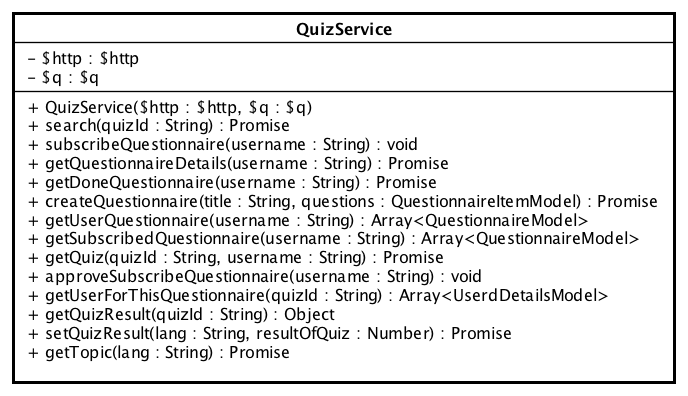
\includegraphics[scale=0.80]{UML/Classi/Front-End/QuizziPedia_Front-end_Services_QuizService.png}
	\caption{QuizziPedia::Front-End::Services::QuizService}
\end{figure}\FloatBarrier
\begin{itemize}
	\item \textbf{Descrizione}: questa classe permette di ottenere i dati di un quiz tramite delle parole chiave inserite dall'utente nella barra di ricerca. Permette inoltre di iscriversi ad un questionario e di scaricare l'intera lista di domande di un questionario a partire dal suo id univoco;
	\item \textbf{Utilizzo}: fornisce le funzionalità per ottenere i dati di un quiz in seguito ad una ricerca dell'utente, passando i risultati ai controllers. Ritorna dei riferimenti alle domande del quiz;
	\item \textbf{Relazione con altre classi:}
	\begin{itemize}
		\item \textit{IN} \texttt{QuestionnaireModel}: rappresenta un questionario. Contiene tutte le informazioni necessarie alla
		presentazione del contenuto del questionario; 
		\item \textit{OUT} \texttt{SearchController}: questa classe permette di gestire la ricerca di questionari e utenti all'interno dell'applicazione;
		\item \textit{OUT} \texttt{QuestionsController}: questa classe permette di gestire il recupero delle domande per poterle stampare nella modalità allenamento;
		\item \textit{OUT} \texttt{QuestionnaireDetailsController}: questa classe permette di gestire i dettagli di un questionario;
		\item \textit{OUT} \texttt{FillingQuestionnaireController}: questa classe permette di gestire la compilazione del questionario;
		\item \textit{OUT} \texttt{CreateQuestionnaireController}: questa classe permette di gestire la creazione di un questionario;
		\item \textit{OUT} \texttt{RegistrationManagementController}: questa classe permette di gestire le iscrizione degli utenti ai questionari;
		\item \textit{OUT} \texttt{ResultsController}: questa classe permette di gestire le iscrizione degli utenti ai questionari; 
		\item \textit{OUT} \texttt{QuestionnaireManagementController}: questa classe permette di gestire tutti i questionari creati da un utente. 
		
	\end{itemize}
	\item \textbf{Attributi:}
	\begin{itemize}
		\item \texttt{-} \texttt{\$http: \$http} \\ Campo dati che contiene un riferimento al servizio \$http che permette la comunicazione con il protocollo \textit{HTTP\ped{G}};
		\item \texttt{-} \texttt{\$q: \$q} \\ Campo dati che contiene un riferimento a \$q, un servizio offerto da \textit{AngularJS\ped{G}} per la gestione, tramite \textit{Promise\ped{G}}, di chiamate asincrone.
	\end{itemize}
	\item \textbf{Metodi:} 
	\begin{itemize}
		\item \texttt{+} \texttt{QuizService(\$http: \$http, \$q: \$q)} \\ Metodo costruttore della classe. \\
		\textbf{Parametri}:
		\begin{itemize}
			\item \texttt{\$http: \$http} \\ Campo dati che contiene un riferimento al servizio \$http che permette la comunicazione con il protocollo \textit{HTTP\ped{G}};
			\item \texttt{\$q: \$q} \\ Campo dati che contiene un riferimento a \$q, un servizio offerto da \textit{AngularJS\ped{G}} per la gestione, tramite \textit{Promise\ped{G}}, di chiamate asincrone. 
		\end{itemize}
	\item \texttt{+} \texttt{search(quizId: String): Promise} \\Metodo che serve per recuperare i questionari dopo averne selezionato uno dalla lista ottenuta da una ricerca. Il metodo ritorna una \textit{Promise\ped{G}}. In caso la \textit{Promise\ped{G}} venga rifiutata, verrà restituito al \texttt{SearchController} un oggetto \texttt{ErrorModelInfo} contenente tutti i dettagli dell'errore. In caso la \textit{Promise\ped{G}} venga accettata, verrà restituito al chiamante del metodo il risultato della chiamata.\\
	\textbf{Parametri}:
	\begin{itemize}
		\item \texttt{quizId: String} \\ Parametro che rappresenta il questionario da cercare.
	\end{itemize}
	\item \texttt{+} \texttt{subscribeQuestionnaire(quizId: String, username: String): Void} \\Metodo per iscriversi ad un questionario;
	\begin{itemize}
		\item \texttt{quizId: String} \\ Parametro che rappresenta il questionario in cui iscrivere l'utente;
		\item \texttt{username: String} \\ Parametro che rappresenta l'utente da registrare al questionario.
	\end{itemize}
	\item \texttt{+} \texttt{getQuestionnaireDetails(username: String): Promise} \\Metodo che serve per ritornare i dettagli di tutti i questionari creati da un utente; Il metodo ritorna una \textit{Promise\ped{G}}. In caso la \textit{Promise\ped{G}} venga rifiutata, verrà restituito al \texttt{StatisticsController} un oggetto \texttt{ErrorModelInfo} contenente tutti i dettagli dell'errore. In caso la \textit{Promise\ped{G}} venga accettata, verrà restituito al chiamante del metodo il risultato della chiamata.\\ 
     \textbf{Parametri}:
	\begin{itemize}
		\item \texttt{username: String} \\ Parametro che rappresenta l'utente del quale andranno caricati tutti i questionari.
	\end{itemize}
	\item \texttt{+ getDoneQuestionnaire(username: String): Promise} \\ Metodo che restituisce tutti i questionari svolti da un utente. Il metodo ritorna una \textit{Promise\ped{G}}. In caso la \textit{Promise\ped{G}} venga rifiutata, verrà restituito al \texttt{UserDetailsController} un oggetto \texttt{ErrorModelInfo} contenente tutti i dettagli dell'errore. \\
	\textbf{Parametri}: 
	\begin{itemize}
		\item \texttt{username: String} \\ Parametro che rappresenta l'utente del quale andranno caricati tutti i questionari svolti.
	\end{itemize}
	\item \texttt{+ createQuestionnaire(title: String, questions: QuestionnaireItemModel): Promise} \\ Metodo che permette di creare un nuovo questionario. Il metodo ritorna una \textit{Promise\ped{G}}. In caso la \textit{Promise\ped{G}} venga rifiutata, verrà restituito al \texttt{CreateQuestionnaireController} un oggetto \texttt{ErrorModelInfo} contenente tutti i dettagli dell'errore. In caso la \textit{Promise\ped{G}} venga accettata, verrà restituito al chiamante del metodo il risultato della chiamata.\\
	\textbf{Parametri}:
	\begin{itemize}
		\item \texttt{title: String} \\ Parametro che rappresenta il titolo del questionario.
		\item \texttt{questions: QuestionnaireItemModel} \\ Parametro contenente tutte le domande del questionario.
	\end{itemize}
	\item \texttt{+} \texttt{getUserQuestionnaire(username: String): QuestionnaireModel[]} \\Metodo che ritorna un array di QuestionnaireModel che sono tutti i questionari creati dall'utente in input.\\
	\textbf{Parametri}:
	\begin{itemize}
		\item \texttt{username: String} \\ Parametro che indica l'identificativo dell'utente del quale vogliamo richiedere i questionari.
	\end{itemize}
	\item \texttt{+} \texttt{getSubscribedQuestionnaire(username: String): QuestionnaireModel[]}: \\Metodo che ritorna la lista dei questionari a cui l'utente è iscritto.\\
	\textbf{Parametri}:
	\begin{itemize}
		\item \texttt{username: String} \\ Parametro che indica l'utente del quale scaricare i quiz a cui risulta iscritto.
	\end{itemize}
	\item \texttt{+ approveSubscribeQuestionnaire(username: String): void} \\ Metodo che approva l'iscrizione di un determinato utente ad un quesitonario.
	\textbf{Parametri}:
	\begin{itemize}
		\item \texttt{username: String} \\ Parametro che indica l'utente da abilitare ad un questionario.
	\end{itemize}
	\item \texttt{getUserForThisQuestionnaire(quizId: String): Array} \\ Metodo che ritorna tutti gli utenti che hanno eseguito il questionario.
	\textbf{Parametri}:
	\begin{itemize}
		\item \texttt{quizId: String} \\ Paramentro che indica il questionario del quale scaricare gli utenti.
	\end{itemize}
	\item \texttt{+ getQuizResults(quizId: String): Object} \\ Metodo che ritorna i risultati di un questionario.
	\textbf{Parametri}:
	\begin{itemize}
		\item \texttt{quiId: String} \\ Id del questionario del quale recuperare i risultati.
	\end{itemize}
	\item \texttt{+ getQuiz(quizId: String, username: String): Promise} \\ Metodo che ritorna una \textit{Promise\ped{G}}. In caso la \textit{Promise\ped{G}} venga rifiutata, verrà restituito al \texttt{CreateQuestionnaireController} un oggetto \texttt{ErrorModelInfo} contenente tutti i dettagli dell'errore. In caso la \textit{Promise\ped{G}} venga accettata, cioè se l'utente è registrato, verrà restituito al chiamante il questionario. \\
	\textbf{Parametri}:
	\begin{itemize}
		\item \texttt{quiId: String} \\ Id del questionario del quale recuperare i risultati.
	\end{itemize}
\end{itemize}
\end{itemize}
\paragraph{QuizziPedia::Front-End::Services::SearchService}

\label{QuizziPedia::Front-End::Services::SearchService}
\begin{figure}[ht]
	\centering
	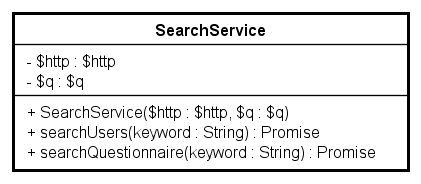
\includegraphics[scale=0.80]{UML/Classi/Front-End/QuizziPedia_Front-end_Services_SearchService.png}
	\caption{QuizziPedia::Front-End::Services::SearchService}
\end{figure}\FloatBarrier
\begin{itemize}
	\item \textbf{Descrizione}: questa classe permette di gestire il recupero dei dati dal back-end a seguito di una ricerca effettuata da un utente;
	\item \textbf{Utilizzo}: fornisce le funzionalità per recuperare dal back-end delle informazioni basandosi sulle \textit{keyword\ped{G}} inserite dall'utente;
	\item \textbf{Relazione con altre classi:}
	\begin{itemize}
		\item \textbf{OUT \texttt{SearchController}}: questa classe permette di gestire la ricerca di questionari e utenti all'interno dell'applicazione.
	\end{itemize}
	\item \textbf{Attributi}:
	\begin{itemize}
		\item \texttt{-} \texttt{\$http: \$http} \\ Campo dati che contiene un riferimento al servizio \$http che permette la comunicazione con il protocollo \textit{HTTP\ped{G}};
		\item \texttt{-} \texttt{\$q: \$q} \\ Campo dati che contiene un riferimento a \$q, un servizio offerto da \textit{Angular\ped{G}} per la gestione, tramite \textit{Promise\ped{G}}, di chiamate asincrone. 
	\end{itemize}
	\item \textbf{Metodi}:
	\begin{itemize}
		\item \texttt{+} \texttt{SearchService(\$http: \$http, \$q: \$q)} \\ Metodo costruttore della classe; \\
		\textbf{Parametri}:
		\begin{itemize}
			\item \texttt{\$http: \$http} \\ Campo dati contenente un riferimento al servizio \$http creato da \textit{Angular\ped{G}} per facilitare la comunicazione mediante protocollo \textit{HTTP\ped{G}};
			\item \texttt{\$q: \$q} \\ Campo dati contenente un riferimento al servizio \$q creato da \textit{Angular\ped{G}} per facilitare la gestione di funzione asincrone mediante l’utilizzo delle \textit{Promise\ped{G}}.
		\end{itemize}
		\item \texttt{+} \texttt{searchUsers(keyword: String): Promise} \\Metodo che serve per recuperare la lista di utenti dopo una ricerca. Il metodo ritorna una \textit{Promise\ped{G}}. In caso la \textit{Promise\ped{G}} venga rifiutata, verrà restituito al \\ \texttt{SearchController} un oggetto \texttt{ErrorModelInfo} contenente tutti i dettagli dell'errore. In caso la \textit{Promise\ped{G}} venga accettata, verrà restituito al chiamante del metodo il risultato della chiamata;\\
		\textbf{Parametri}:
		\begin{itemize}
			\item \texttt{keyword: String} \\ Parametro che rappresenta la parola da cercare.
		\end{itemize}
		\item \texttt{+} \texttt{searchQuestionnaire(keyword: String): Promise} \\Metodo che serve per recuperare la lista dei questionari dopo una ricerca. Il metodo ritorna una \textit{Promise\ped{G}}. In caso la \textit{Promise\ped{G}} venga rifiutata, verrà restituito al \texttt{SearchController} un oggetto \texttt{ErrorModelInfo} contenente tutti i dettagli dell'errore. In caso la \textit{Promise\ped{G}} venga accettata, verrà restituito al chiamante del metodo il risultato della chiamata.\\
		\textbf{Parametri}:
		\begin{itemize}
			\item \texttt{keyword: String} \\ Parametro che rappresenta la parola da cercare.
		\end{itemize}
	\end{itemize}
\end{itemize}
\paragraph{QuizziPedia::Front-End::Services::StatisticsService}
\begin{figure}[ht]
	\centering
	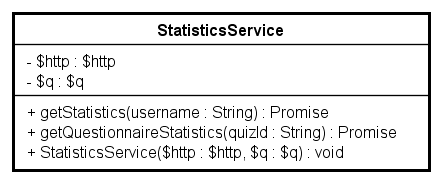
\includegraphics[scale=0.60]{UML/Classi/Front-End/QuizziPedia_Front-end_Services_StatisticsService.png}
	\caption{QuizziPedia::Front-End::Services::StatisticsService}
\end{figure}\FloatBarrier
\begin{itemize}
	\item \textbf{Descrizione}: questa classe permette di ottenere le statistiche dell'utente;
	\item \textbf{Utilizzo}: fornisce al controller le statistiche salvate;
	\item \textbf{Relazione con altre classi}:
	\begin{itemize}
		\item \textit{IN} \texttt{StatisticsController}: questa classe permette di le statistiche di un utente.
	\end{itemize}
	\item \textbf{Attributi:}
	\begin{itemize}
		\item \texttt{-} \texttt{\$http: \$http} \\ Campo dati che contiene un riferimento al servizio \$http che permette la comunicazione con il protocollo \textit{HTTP\ped{G}};
		\item \texttt{-} \texttt{\$q: \$q} \\ Campo dati che contiene un riferimento a \$q, un servizio offerto da \textit{AngularJS\ped{G}} per la gestione, tramite \textit{Promise\ped{G}}, di chiamate asincrone.
	\end{itemize}
	\item \textbf{Metodi:}
	\begin{itemize}
		\item \texttt{+} \texttt{StatisticsService(\$http: \$http, \$q: \$q)} \\ Metodo costruttore della classe \\
		\textbf{Parametri}:
		\begin{itemize}
			\item \texttt{-} \texttt{\$http: \$http} \\ Campo dati che contiene un riferimento al servizio \$http che permette la comunicazione con il protocollo \textit{HTTP\ped{G}};
			\item \texttt{-} \texttt{\$q: \$q} \\ Campo dati che contiene un riferimento a \$q, un servizio offerto da \textit{AngularJS\ped{G}} per la gestione, tramite \textit{Promise\ped{G}}, di chiamate asincrone.
		\end{itemize}
		\item \texttt{+} \texttt{getStatistics(username: String): Promise}: \\Metodo che serve per recuperare le statistiche di un utente tramite chiamata al back-end. Il metodo ritorna una \textit{Promise\ped{G}}. In caso la \textit{Promise\ped{G}} venga rifiutata, verrà restituito al \texttt{StatisticsController} un oggetto \texttt{ErrorModelInfo} contenente tutti i dettagli dell'errore. In caso la \textit{Promise\ped{G}} venga accettata, verrà restituito al chiamante del metodo il risultato della chiamata.\\
	    \textbf{Parametri}:
		\begin{itemize}
			\item \texttt{username: String} \\ Parametro che indica l'utente del quale andranno caricate tutte le statistiche.
		\end{itemize}
		\item \texttt{+} \texttt{getQuestionnaireStatistics(quizId: String): Promise} \\Metodo che restituisce le statistiche di un questionario.  Il metodo ritorna una \textit{Promise\ped{G}}. In caso la \textit{Promise\ped{G}} venga rifiutata, verrà restituito al \texttt{StatisticsController} un oggetto \texttt{ErrorModelInfo} contenente tutti i dettagli dell'errore. In caso la \textit{Promise\ped{G}} venga accettata, verrà restituito al chiamante del metodo il risultato della chiamata.\\
		\textbf{Parametri}:
		\begin{itemize}
			\item \texttt{quizId: String} \\ Parametro che indica il questionario del quale verranno caricate le statistiche.
		\end{itemize}
	\end{itemize}
\end{itemize}
\paragraph{QuizziPedia::Front-End::Services::UserDetailsService}
\begin{figure}[ht]
	\centering
	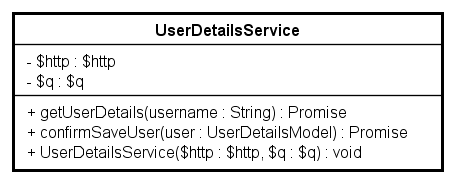
\includegraphics[scale=0.60]{UML/Classi/Front-End/QuizziPedia_Front-end_Services_UserDetailsService.png}
	\caption{QuizziPedia::Front-End::Services::UserDetailsService}
\end{figure}\FloatBarrier
\begin{itemize}
	\item \textbf{Descrizione}: questa classe permette di ottenere i dati personali degli utenti;
	\item \textbf{Utilizzo}: utilizzata per ottenere i dati personali di un utente. Permette inoltre di trovare i dati di utenti ricercati tramite l'apposita barra di ricerca;
	\item \textbf{Relazione con altre classi}:
	\begin{itemize}
		\item \textit{IN} \texttt{UserDetailsModel}: rappresenta un utente. Contiene tutte le informazioni necessarie alla
		presentazione del contenuto di un utente sia nella visualizzazione che nella gestione di un profilo; 
		\item \textit{OUT} \texttt{SearchController}: questa classe permette di gestire la ricerca di questionari e utenti all'interno dell'applicazione;
		\item \textit{OUT} \texttt{UserDetailsController}: questa classe permette di gestire i dati di un utente;
		\item \textit{OUT} \texttt{ProfileManagementController}: questa classe permette di gestire il profilo personale di un utente. 
	\end{itemize}
	\item \textbf{Attributi:}
	\begin{itemize}
		\item \texttt{-} \texttt{\$http: \$http} \\ Campo dati che contiene un riferimento al servizio \$http che permette la comunicazione con il protocollo \textit{HTTP\ped{G}};
		\item \texttt{-} \texttt{\$q: \$q} \\ Campo dati che contiene un riferimento a \$q, un servizio offerto da \textit{AngularJS\ped{G}} per la gestione, tramite \textit{Promise\ped{G}}, di chiamate asincrone.
	\end{itemize}
	\item \textbf{Metodi:}
	\begin{itemize}
		\item \texttt{+} \texttt{UserDetailsService(\$http: \$http, \$q: \$q)} \\ Metodo costruttore della classe. \\
		\textbf{Parametri}:
		\begin{itemize}
			\item \texttt{-} \texttt{\$http: \$http} \\ Campo dati che contiene un riferimento al servizio \$http che permette la comunicazione con il protocollo \textit{HTTP\ped{G}};
			\item \texttt{-} \texttt{\$q: \$q} \\ Campo dati che contiene un riferimento a \$q, un servizio offerto da \textit{AngularJS\ped{G}} per la gestione, tramite \textit{Promise\ped{G}}, di chiamate asincrone.
		\end{itemize}
		\item \texttt{+} \texttt{getUserDetails(username: String): Promise} \\ Metodo che serve per ottenere i dettagli di un utente. Il metodo ritorna una \textit{Promise\ped{G}}. In caso la \textit{Promise\ped{G}} venga rifiutata, verrà restituito al \texttt{SearchController} un oggetto \texttt{ErrorModelInfo} contenente tutti i dettagli dell'errore. In caso la \textit{Promise\ped{G}} venga accettata, verrà restituito al chiamante del metodo il risultato della chiamata.\\
		\textbf{Parametri}:
		\begin{itemize}
			\item \texttt{username: String} \\ Parametro che indica l'utente del quale andranno caricati tutti i dati personali.
		\end{itemize}
		\item \texttt{+} \texttt{confirmSaveUser(user: Object, imageObject: Object): Promise} \\Metodo che serve per inviare al back-end una richiesta di salvataggio persistente dei dati. Viene invocato da Confirm in ProfileManagementController. Il metodo ritorna una \textit{Promise\ped{G}}. In caso la \textit{Promise\ped{G}} venga rifiutata, verrà restituito al \texttt{ProfileManagementController} un oggetto \texttt{ErrorModelInfo} contenente tutti i dettagli dell'errore. In caso la \textit{Promise\ped{G}} venga accettata, verrà restituito al chiamante del metodo il risultato della chiamata.\\
		\textbf{Parametri}:
		\begin{itemize}
			\item \texttt{user: Object} \\ Parametro che indica l'oggetto contenente tutti i dati dell'utente che dovranno essere salvati dal back-end;
			\item \texttt{+ imageObject: Object} \\ Oggetto contenente i seguenti attributi: \texttt{+ imageUrl: String}, \texttt{+ image: Object};
		\end{itemize}
	
	\end{itemize}
\end{itemize}

